\documentclass[12pt,a4paper,oneside]{report}
% ============================================================
% PREAMBLE -- Rapport de stage PFA1 (format UM6P)
% Police Carlito (clone metrique libre de Calibri), taille 12.
% Compiler avec XeLaTeX / tectonic.
% ============================================================

\usepackage[french]{babel}
\usepackage[margin=2.4cm, top=2.6cm, bottom=2.4cm]{geometry}

% ------------------------------------------------------------
% POLICE : Carlito = clone metrique libre de Calibri
% ------------------------------------------------------------
\usepackage{fontspec}
\setmainfont{Carlito}[
  Extension      = .ttf,
  Path           = /usr/share/fonts/carlito/,
  UprightFont    = Carlito-Regular,
  BoldFont       = Carlito-Bold,
  ItalicFont     = Carlito-Italic,
  BoldItalicFont = Carlito-BoldItalic
]
\setmonofont{DejaVu Sans Mono}[Scale=0.85]

\usepackage{amsmath}
\usepackage{amssymb}

\usepackage{graphicx}
\graphicspath{{../plots/}{./figures/}}

\usepackage{booktabs}
\usepackage{array}
\usepackage{tabularx}
\usepackage{adjustbox}
\usepackage{enumitem}
\usepackage[table]{xcolor}
\usepackage{caption}
\usepackage{float}

\usepackage{tikz}
\usetikzlibrary{arrows.meta, positioning}

\usepackage{fancyhdr}
\usepackage{titlesec}
\usepackage{titletoc}

\usepackage[hidelinks]{hyperref}

% Intitules conformes aux consignes de l'ecole
\addto\captionsfrench{%
  \renewcommand{\listfigurename}{Liste des figures}%
  \renewcommand{\listtablename}{Liste des tableaux}%
  \renewcommand{\bibname}{Références bibliographiques}%
}

% ------------------------------------------------------------
% PALETTE
% ------------------------------------------------------------
\definecolor{accent}{RGB}{17,112,120}      % teal -- titres
\definecolor{caplabel}{RGB}{26,105,150}    % bleu -- etiquettes figures/tables
\definecolor{umorange}{RGB}{215,74,42}     % orange UM6P -- filets
\definecolor{rulegray}{RGB}{120,120,120}

% ------------------------------------------------------------
% LEGENDES : etiquette coloree en gras, texte justifie
% ------------------------------------------------------------
\captionsetup{
  font=small,
  labelfont={bf,color=caplabel},
  labelsep=period,
  justification=justified,
  singlelinecheck=false,
  skip=6pt
}
\captionsetup[figure]{justification=justified}
\captionsetup[table]{justification=justified}

\renewcommand{\arraystretch}{1.15}
\newcolumntype{Y}{>{\centering\arraybackslash}X}
\newcommand{\rowrule}{\midrule[0.2pt]}

% ------------------------------------------------------------
% EN-TETES / PIEDS
% ------------------------------------------------------------
% Chaque style est defini par \fancypagestyle et re-execute son propre corps
% a l'activation : sans cela, le \fancyhf{} du style "plain" efface
% definitivement les en-tetes du style principal (registres globaux fancyhdr).
\setlength{\headheight}{15pt}

\fancypagestyle{main}{%
  \fancyhf{}%
  \renewcommand{\headrulewidth}{0.4pt}%
  \renewcommand{\footrulewidth}{0pt}%
  \fancyhead[L]{\small\nouppercase{\leftmark}}%
  \fancyhead[R]{\small Rapport de stage PFA1}%
  \fancyfoot[C]{\thepage}%
}

\fancypagestyle{plain}{%
  \fancyhf{}%
  \renewcommand{\headrulewidth}{0pt}%
  \renewcommand{\footrulewidth}{0pt}%
  \fancyfoot[C]{\thepage}%
}

\pagestyle{main}

% ------------------------------------------------------------
% TITRES
% ------------------------------------------------------------
\titleformat{\chapter}[display]
  {\normalfont\huge\bfseries\color{accent}}
  {\large\chaptertitlename\ \thechapter}
  {8pt}
  {\Huge}
  [{\color{umorange}\titlerule[1.2pt]}]
\titlespacing*{\chapter}{0pt}{-28pt}{16pt}

\titleformat{\section}
  {\large\bfseries\color{accent}}
  {\thesection}{0.7em}{}
\titlespacing*{\section}{0pt}{2.8ex plus 1ex minus .2ex}{1.2ex plus .2ex}

\titleformat{\subsection}
  {\normalsize\bfseries\color{accent}}
  {\thesubsection}{0.7em}{}
\titlespacing*{\subsection}{0pt}{2.2ex plus 1ex minus .2ex}{0.9ex plus .2ex}

\titleformat{\subsubsection}
  {\normalsize\bfseries}
  {\thesubsubsection}{0.7em}{}
\titlespacing*{\subsubsection}{0pt}{1.8ex plus 1ex minus .2ex}{0.7ex plus .2ex}

% ------------------------------------------------------------
% STYLE TIKZ partage par les schemas
% ------------------------------------------------------------
\tikzset{
  rbox/.style={draw, rounded corners, fill=accent!10, align=center,
               minimum height=1.0cm, text width=#1, font=\small},
  rbox/.default=2.6cm,
  flow/.style={-{Latex[length=2.2mm]}, thick}
}

% ------------------------------------------------------------
% DIVERS
% ------------------------------------------------------------
\setlength{\parskip}{0.42em}
\setlength{\parindent}{0pt}
\setlist{itemsep=2pt, topsep=3pt, parsep=0pt}


\begin{document}

% ============================================================
% PAGE DE GARDE
% ============================================================
\begin{titlepage}
\thispagestyle{empty}
\centering


\includegraphics[width=0.50\textwidth]{um6p_college_of_computing_logo.png}

\vspace{1.0cm}

{\large Université Mohammed VI Polytechnique}\\[2pt]
{\large College of Computing -- Benguerir}\\[2pt]
{\large Filière~: Intelligence Artificielle \& Data Science}

\vspace{1.2cm}

{\Large\bfseries RAPPORT DE STAGE}\\[4pt]
{\large Projet de Fin d'Année 1 (PFA1)}

\vspace{1.0cm}
{\color{rulegray}\rule{0.86\textwidth}{0.8pt}}
\vspace{0.8cm}

{\LARGE\bfseries\color{accent}
Schémas de capture de chocs augmentés par\\[6pt]
apprentissage automatique~: de l'imitation\\[6pt]
à une perte physique déroulée\\}

\vspace{0.8cm}
{\color{rulegray}\rule{0.86\textwidth}{0.8pt}}

\vspace{1.2cm}

{\large Réalisé au sein de}\\[4pt]
{\large\bfseries UM6P -- COLLEGE OF COMPUTING}\\[4pt]
{\large Du 1\textsuperscript{er} juin au 1\textsuperscript{er} août 2026}

\vspace{1.4cm}

\noindent
\begin{minipage}[t]{0.48\textwidth}
\raggedright
{\bfseries Réalisé par~:}\\[3pt]
Yasser BAOUZIL
\end{minipage}
\hfill
\begin{minipage}[t]{0.48\textwidth}
\raggedleft
{\bfseries Encadrant professionnel~:}\\[3pt]
M. Radouan BOUKHARFANE\\[8pt]
{\bfseries Encadrant académique~:}\\[3pt]
M. Radouan BOUKHARFANE
\end{minipage}

\vfill
{\large Année universitaire 2025 -- 2026}

\end{titlepage}

% ============================================================
% FRONT MATTER
% ============================================================
\pagenumbering{roman}
\setcounter{page}{1}
\pagestyle{plain}

\chapter*{Remerciements}
\addcontentsline{toc}{chapter}{Remerciements}
\markboth{Remerciements}{}

Je tiens à exprimer ma sincère gratitude à l'ensemble des personnes qui ont
rendu ce stage possible et formateur.

Je remercie tout particulièrement M.~Radouan Boukharfane, qui a encadré ce
stage à la fois sur le plan professionnel et académique, pour m'avoir confié
une véritable question de recherche plutôt qu'un cahier des charges figé, pour
avoir proposé l'idée centrale de la seconde phase du projet -- la fonction de
perte physique déroulée -- et pour la précision de ses retours, notamment sur
la définition correcte du terme BVD, qui a débloqué une étape clé du travail.

Je remercie également le corps professoral et l'administration du College of
Computing de l'Université Mohammed~VI Polytechnique pour la formation reçue et
pour le cadre de travail mis à disposition durant ces deux mois.

\chapter*{Résumé}
\addcontentsline{toc}{chapter}{Résumé}
\markboth{Résumé}{}

Ce rapport présente le travail réalisé lors de mon stage de fin d'année (PFA1)
au sein du College of Computing de l'Université Mohammed~VI Polytechnique. La
mission portait sur les schémas numériques de capture de chocs augmentés par
apprentissage automatique~: déterminer si un réseau de neurones peut améliorer
la reconstruction d'un schéma classique de type WENO/TENO pour les lois de
conservation hyperboliques.

Le travail s'organise en quatre volets. Le premier reproduit les résultats
publiés du schéma WENO5-NN de Stevens \& Colonius afin d'établir une référence
vérifiée. Le deuxième étend la même approche à TENO5 par entraînement par
imitation, et met en évidence un plafond structurel~: un réseau entraîné à
copier la décision d'un schéma enseignant ne peut, par construction, le
dépasser. Ce constat a motivé la seconde phase du stage, fondée sur une
\emph{fonction de perte physique déroulée} proposée par l'encadrant~: au lieu
d'une étiquette d'imitation, le réseau est déroulé sur $K$ pas de simulation
réels et évalué directement contre la solution vraie. Cette formulation a exigé
une réécriture complète et différentiable du cœur numérique du projet en JAX.
Les troisième et quatrième volets appliquent cette perte aux benchmarks
scalaires (advection, Burgers) puis au système d'Euler (Sod, Shu--Osher).

Le résultat principal est une victoire nette sur les benchmarks canoniques
scalaires ($3{,}5\%$ de gain sur l'advection, $18{,}6\%$ sur Burgers, hors
distribution d'entraînement) et une première victoire franche sur le système
d'Euler ($1{,}84\%$ sur Shu--Osher), obtenues grâce à un mécanisme de mélange
convexe piloté par une tête dédiée. Le second résultat, négatif mais tout aussi
instructif, est que le cas de Sod reste une quasi-égalité défavorable au réseau,
et qu'un balayage direct du coefficient de mélange démontre qu'il s'agit d'une
limite structurelle du schéma appris, non d'un défaut de calibrage.

\vspace{0.6em}
\textbf{Mots-clés~:} schémas WENO/TENO, lois de conservation hyperboliques,
capture de chocs, apprentissage profond, différentiation automatique, JAX,
perte physique déroulée, système d'Euler.

\tableofcontents
\listoffigures
\addcontentsline{toc}{chapter}{Table des figures}
\listoftables
\addcontentsline{toc}{chapter}{Liste des tableaux}


% ============================================================
% CORPS
% ============================================================
\cleardoublepage
\pagenumbering{arabic}
\setcounter{page}{1}
\pagestyle{main}

\chapter*{Introduction}
\addcontentsline{toc}{chapter}{Introduction}
\markboth{Introduction}{}

Dans le cadre de ma première année du cycle ingénieur au College of Computing
de l'Université Mohammed~VI Polytechnique, j'ai effectué un stage de fin
d'année de deux mois, du 1\textsuperscript{er} juin au
1\textsuperscript{er} août 2026, au sein de l'établissement même, sous
l'encadrement de M.~Radouan Boukharfane.

La simulation numérique des écoulements compressibles se heurte à une
difficulté ancienne et structurante~: en présence d'un choc, une solution
discontinue apparaît en temps fini même à partir d'une donnée initiale
parfaitement lisse. Un schéma numérique d'ordre élevé appliqué naïvement
produit alors des oscillations parasites (phénomène de Gibbs) qui peuvent
rendre la solution non physique -- densité ou pression négatives -- et faire
diverger le calcul. Les schémas de la famille ENO/WENO/TENO résolvent ce
problème en adaptant localement la reconstruction~: ils détectent les
sous-stencils traversés par une discontinuité et en réduisent, voire
annulent, la contribution.

Cette détection repose sur des indicateurs de régularité analytiques et sur des
constantes fixées empiriquement. C'est précisément ce point que
l'apprentissage automatique promet d'améliorer~: si la décision
« garder/écarter » d'un schéma classique est une fonction non linéaire des
valeurs locales de la solution, un réseau de neurones peut en principe
l'approcher, voire faire mieux. Plusieurs travaux publiés ont exploré cette
voie, avec des résultats encourageants mais contrastés.

La question posée à ce stage était donc la suivante~: \emph{un réseau de
neurones peut-il réellement surpasser un schéma classique de capture de chocs,
mesuré contre la solution vraie et sur des benchmarks canoniques~?} Ce rapport
répond à cette question en quatre volets expérimentaux, et documente aussi bien
les résultats positifs que les échecs, ces derniers ayant orienté de manière
décisive la suite du travail.

Le rapport s'organise comme suit. Le chapitre~\ref{chap:entreprise} présente
l'établissement d'accueil. Le chapitre~\ref{chap:contexte} expose le contexte
scientifique, le périmètre du projet et la méthodologie adoptée. Le
chapitre~\ref{chap:conception} décrit la conception de la solution, depuis
l'architecture du réseau jusqu'à la réécriture différentiable en JAX. Le
chapitre~\ref{chap:realisation} détaille les quatre volets expérimentaux. Le
chapitre~\ref{chap:resultats} consolide les résultats et en propose une analyse
critique.

% ============================================================
\chapter{Présentation de l'établissement d'accueil}
\label{chap:entreprise}

\section{Domaine d'activité}

L'Université Mohammed~VI Polytechnique (UM6P) est un établissement
d'enseignement supérieur et de recherche marocain, implanté principalement sur
le campus de Benguerir, dans la région de Marrakech-Safi. Orientée vers la
recherche appliquée et l'innovation, elle couvre un large spectre de domaines
allant des sciences des matériaux et de l'agriculture aux sciences du numérique.

Le stage s'est déroulé au sein du \textbf{College of Computing}, l'une des
composantes de l'université, dédiée aux sciences et technologies de
l'information~: informatique, intelligence artificielle, science des données et
calcul scientifique. À la différence d'une entreprise, la finalité première de
cette structure n'est pas la production d'un service commercial mais la
production de connaissances~: publications scientifiques, encadrement doctoral,
et développement d'outils et de méthodes réutilisables par la communauté
scientifique.

Le projet mené durant ce stage s'inscrit dans l'axe du \emph{calcul
scientifique et de la mécanique des fluides numérique} (CFD), à l'intersection
de l'analyse numérique classique et de l'apprentissage automatique -- un
domaine en forte expansion, où les méthodes d'apprentissage sont utilisées non
pas pour remplacer les solveurs numériques, mais pour en améliorer des
composants ciblés.

\section{Structure organisationnelle}

L'UM6P est organisée en \emph{colleges} et instituts thématiques, chacun
regroupant des programmes d'enseignement et des équipes de recherche autour
d'un domaine. Le College of Computing suit cette logique~: il associe une
mission d'enseignement (formations d'ingénieurs, dont la filière Intelligence
Artificielle \& Data Science que je suis) et une mission de recherche organisée
en équipes rattachées à des enseignants-chercheurs.

L'encadrement d'un stagiaire y suit un schéma direct, sans hiérarchie
intermédiaire~: l'étudiant est rattaché à un enseignant-chercheur qui définit le
sujet, oriente le travail et en évalue les résultats. Dans mon cas,
M.~Radouan Boukharfane a assuré simultanément le rôle d'encadrant professionnel
et d'encadrant académique. Cette organisation a une conséquence pratique
importante sur le déroulement du stage~: le pilotage s'est fait par objectifs
scientifiques et par validation de résultats mesurés, plutôt que par jalons de
livraison.

\section{Métiers présents}

Les métiers représentés dans l'environnement immédiat du stage relèvent
principalement de la recherche et du calcul scientifique~:

\begin{itemize}
  \item \textbf{Enseignant-chercheur} -- définit les axes de recherche, encadre
  et publie. C'est le métier de mon encadrant.
  \item \textbf{Doctorant / chercheur postdoctoral} -- conduit un programme de
  recherche sur plusieurs années.
  \item \textbf{Ingénieur de recherche / calcul scientifique} -- implémente et
  optimise les codes de simulation, assure la reproductibilité des expériences.
  \item \textbf{Data scientist / ingénieur en apprentissage automatique} --
  conçoit, entraîne et évalue les modèles~; profil vers lequel ma formation me
  destine, et qui correspond à la nature hybride du sujet traité.
\end{itemize}

Le travail réalisé durant ce stage se situe précisément à l'intersection des
deux derniers métiers~: il a exigé autant la maîtrise d'un solveur numérique
(schémas de reconstruction, intégration temporelle, stabilité) que celle d'une
chaîne d'apprentissage (conception d'architecture, fonction de perte,
entraînement, évaluation).

% ============================================================
\chapter{Contexte scientifique et cadrage du projet}
\label{chap:contexte}

\section{Contexte scientifique~: volumes finis et lois de conservation}
\label{sec:fond-vf}

Une loi de conservation hyperbolique scalaire s'écrit
\[
\partial_t u + \partial_x f(u) = 0,
\]
et le système d'Euler compressible en est la généralisation vectorielle, où
$u$ regroupe les variables conservées (densité, quantité de mouvement, énergie)
et $f(u)$ le flux physique associé. Les deux sont résolus ici par la méthode
des lignes~: le domaine est divisé en $N$ cellules, chaque cellule $i$ stocke
une moyenne $u_i$, et l'équation est avancée en estimant le flux à chaque
interface $i+1/2$ puis en intégrant
\[
\frac{d u_i}{dt} = -\frac{1}{\Delta x}\left(\hat f_{i+1/2} - \hat f_{i-1/2}\right)
\]
en temps, à l'aide d'un intégrateur de Runge--Kutta d'ordre trois (SSPRK3).
Cet intégrateur a la propriété d'être une combinaison convexe de pas d'Euler
explicite, ce qui garantit qu'il n'amplifie pas un état déjà non oscillant. Le
flux est par ailleurs séparé en une partie amont et une partie aval
(séparation de Lax--Friedrichs) avant reconstruction, afin que le
décentrement reste bien défini même là où la vitesse d'onde change de signe.

Toute la difficulté numérique réside dans $\hat f_{i+1/2}$~: reconstruire une
estimation d'ordre élevé à l'interface sans introduire d'oscillations près
d'une discontinuité. Pour le système d'Euler, la reconstruction est appliquée
non pas aux variables conservées directement, mais aux \emph{champs
caractéristiques} du système, obtenus par un changement de base local qui
découple les trois ondes. Ce détail a une conséquence importante pour la
suite~: ce changement de base dépend de la solution elle-même, si bien qu'une
reconstruction imparfaite dégrade la base utilisée au pas suivant
(section~\ref{sec:instabilite}).

\section{Reconstructions ENO, WENO et TENO}
\label{sec:fond-schemas}

Les trois schémas reconstruisent $\hat f_{i+1/2}$ à partir du même stencil à
5~points $f_{i-2},\dots,f_{i+2}$, découpé en trois sous-stencils candidats de
3~points qui se chevauchent. Chaque candidat fournit, par interpolation
polynomiale, sa propre estimation de la valeur à l'interface. Ce qui distingue
les trois schémas est uniquement la \emph{façon} de combiner ces trois
estimations.

\textbf{ENO} \cite{harten1987} retient le seul candidat le plus régulier et
écarte les deux autres. Ce choix étant discontinu par rapport aux données, il
limite l'ordre de précision atteignable dans les régions lisses.

\textbf{WENO} \cite{jiang1996} remplace ce choix dur par une combinaison
convexe des trois candidats~:
\[
\hat f_{i+1/2} = \sum_{k=0}^{2} w_k\, \hat f_{k,i+1/2}, \qquad
w_k = \frac{\alpha_k}{\sum_{l}\alpha_l}, \qquad
\alpha_k = \frac{d_k}{(\beta_k + \varepsilon)^{q}} .
\]
Les $d_k$ sont des poids fixes, dits \emph{optimaux}, qui font retrouver la
reconstruction complète d'ordre cinq lorsque les trois candidats s'accordent~;
$\varepsilon$ évite la division par zéro. Chaque $\beta_k$ est un
\textbf{indicateur de régularité}~: une somme de différences finies au carré
qui mesure à quel point le candidat $k$ est « agité ». Le mécanisme tient en
une phrase~: près d'une discontinuité, le candidat qu'elle traverse a un
$\beta_k$ grand, donc un poids $w_k$ qui s'effondre vers zéro~; en région
lisse, tous les $\beta_k$ sont petits et comparables, $w_k \to d_k$, et
l'ordre cinq est retrouvé.

\textbf{TENO} \cite{fu2016} conserve ce mécanisme mais remplace la pondération
progressive par une décision \emph{binaire}. Les $\beta_k$ sont d'abord
normalisés en une mesure $\chi_k \in [0,1]$, puis comparés à un seuil fixe
$C_T$~:
\[
\delta_k = \begin{cases} 0, & \text{si } \chi_k < C_T \quad (\text{candidat écarté}) \\[2pt]
                         1, & \text{sinon} \quad (\text{candidat gardé}), \end{cases}
\qquad
w_k = \frac{d_k\,\delta_k}{\sum_{l}d_l\,\delta_l} .
\]
Un candidat sous le seuil est donc écarté \emph{complètement} plutôt que
simplement sous-pondéré. C'est ce qui donne à TENO5 une capture des
discontinuités plus nette que WENO5, à coût de calcul comparable, et c'est
pourquoi c'est ce schéma que le stage cherche à améliorer.

\textbf{C'est la décision $\delta_k$ que ce stage entraîne un réseau de
neurones à remplacer}~: à partir du stencil normalisé à 5~points, produire pour
chacun des trois candidats la probabilité qu'il doive être écarté.

\section{De l'écoulement réel au signal unidimensionnel}

Un choc n'est pas une abstraction mathématique~: c'est une discontinuité
physique observable. Le panneau~(a) de la figure~\ref{fig:pipeline} en donne
une image directe -- une photographie schlieren d'un T-38 en vol supersonique
à Mach~1,1, prise par la NASA \cite{nasa1993}. La technique schlieren rend
visibles les gradients de densité de l'air~: les bandes sombres obliques sont
les ondes de choc attachées à l'appareil.

En prélevant une \textbf{coupe unidimensionnelle} à travers cet écoulement
(trait rouge), on obtient le signal $u(x)$ du panneau~(b)~: de longues zones
régulières séparées par quelques transitions très raides. C'est exactement la
structure que les schémas ENO/WENO/TENO sont conçus pour traiter, et c'est
aussi ce qui rend le problème difficile~: un schéma d'ordre élevé est excellent
sur les zones régulières et catastrophique au voisinage des transitions, où il
produit des oscillations parasites.

Tout le travail de ce stage porte donc sur une seule question, posée sur ce
signal 1D~: \emph{comment reconstruire la valeur à l'interface entre deux
cellules, avec un ordre élevé là où le signal est régulier, sans osciller là où
il ne l'est pas~?}

\medskip
La figure~\ref{fig:pipeline} déroule la chaîne complète sur ce cas réel,
depuis l'écoulement physique jusqu'à l'avancement en temps. Les deux premières
étapes constituent une mise en place effectuée une seule fois~; les suivantes forment
la boucle répétée à chaque pas de temps.

\begin{figure}[H]
\centering
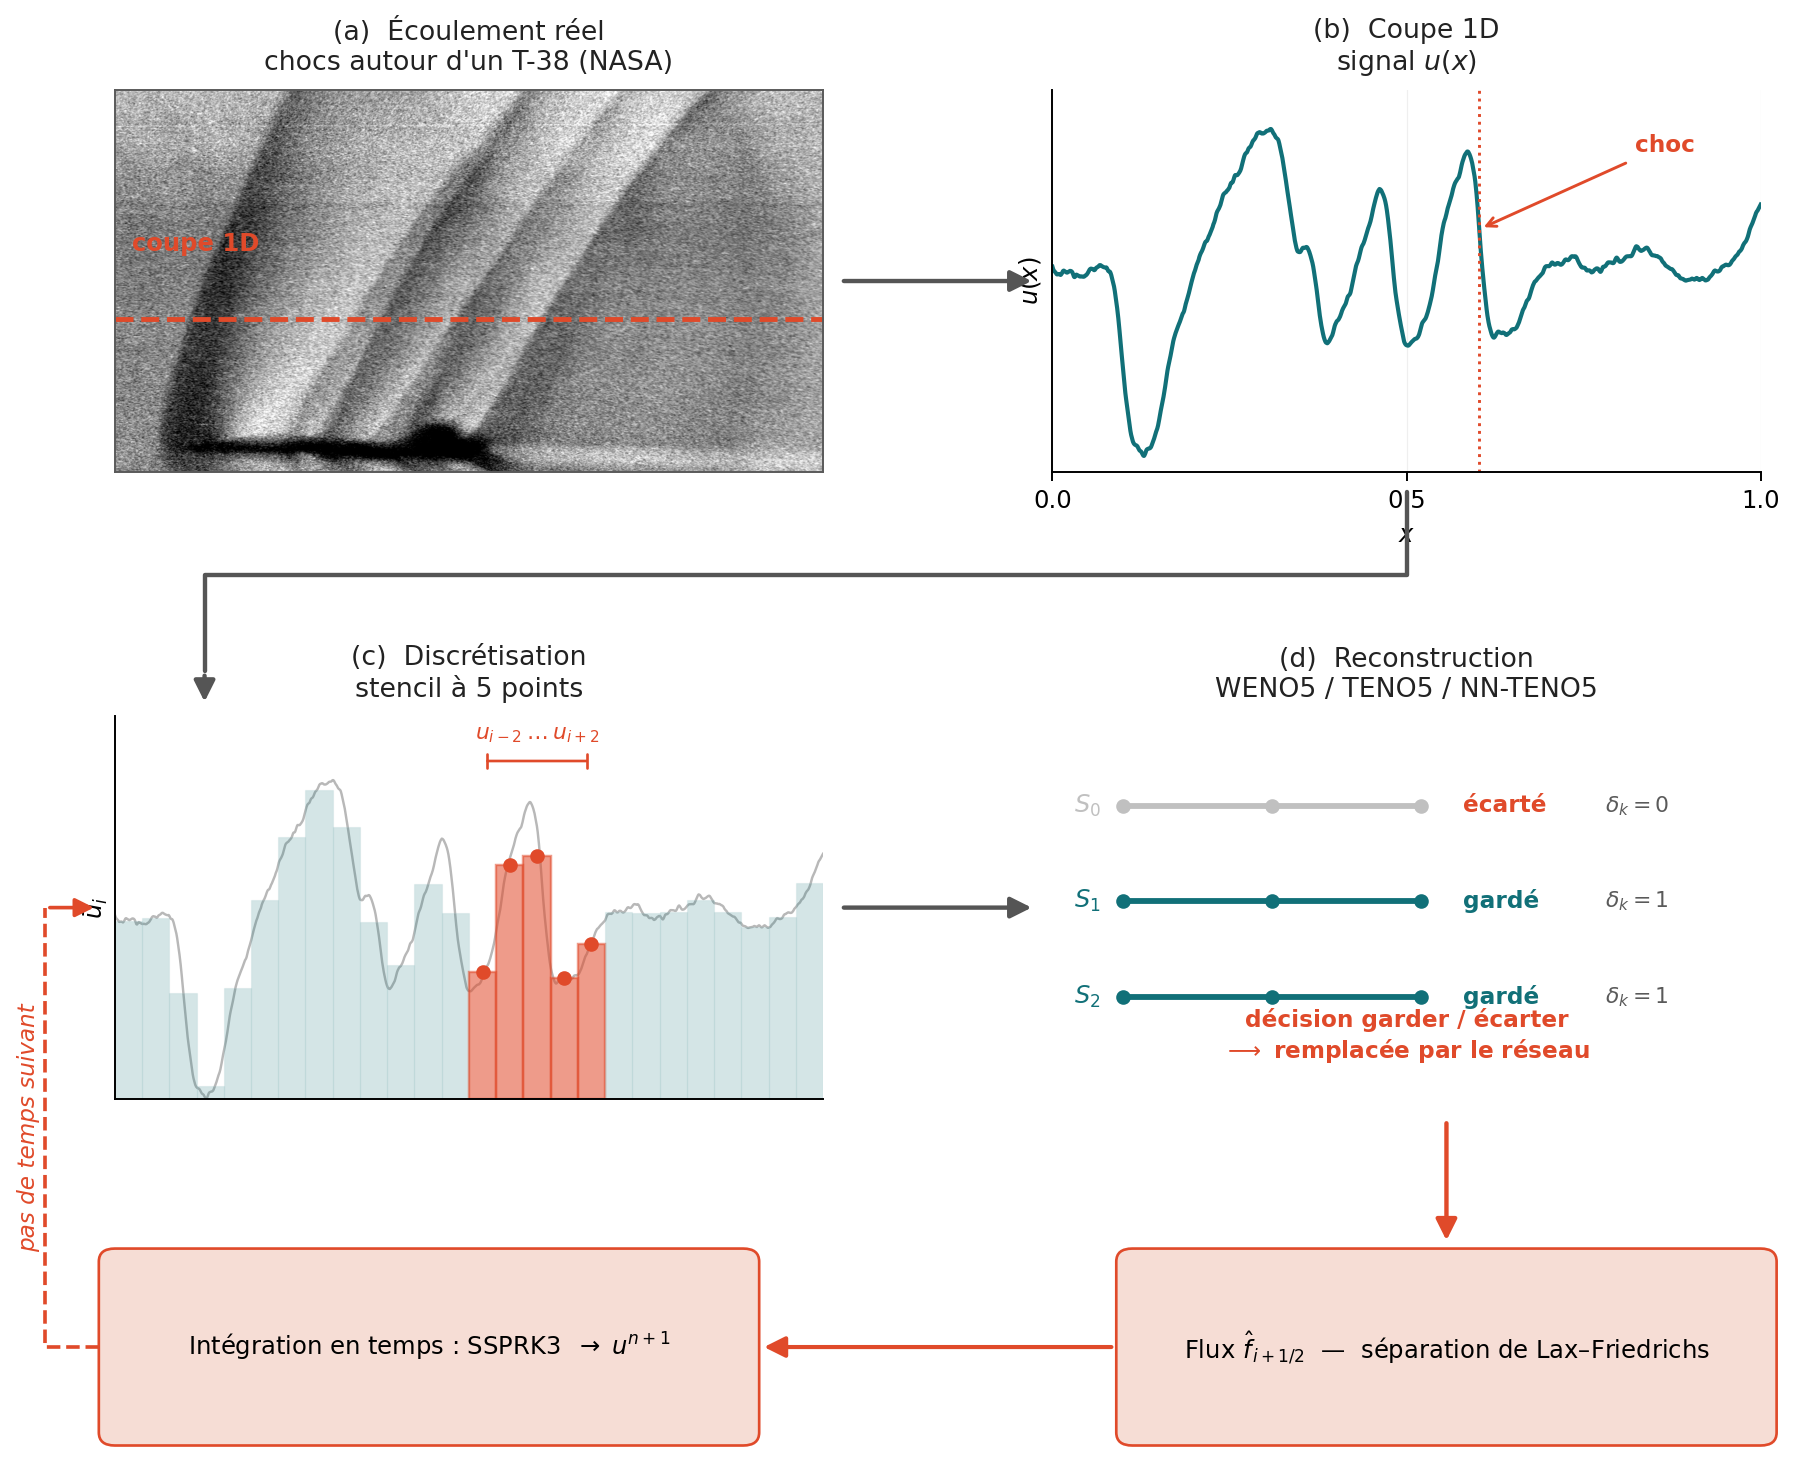
\includegraphics[width=\textwidth]{pipeline_visuel.png}
\caption{Chaîne de calcul complète, illustrée sur un cas réel. (a) Ondes de
choc autour d'un T-38 en vol supersonique (photographie schlieren,
NASA~\cite{nasa1993}) et trace de la coupe~1D. (b) Signal $u(x)$ effectivement
extrait des pixels le long de cette coupe~; le repère marque la transition la
plus raide. (c) Discrétisation en cellules et stencil à 5~points centré sur ce
front. (d) Les trois candidats de TENO5~: celui que la discontinuité traverse
est écarté ($\delta_k = 0$), les autres sont conservés. Le flux reconstruit
alimente ensuite la séparation de Lax--Friedrichs puis l'intégrateur SSPRK3, et
la boucle reprend au pas suivant. \textbf{Le stage porte exclusivement sur la
décision du panneau~(d)}~; tous les autres maillons sont identiques entre le
schéma classique et le schéma appris.}
\label{fig:pipeline}
\end{figure}

Le point important est que \textbf{le réseau n'intervient qu'à une seule
étape}. Il ne remplace ni l'intégrateur temporel, ni la séparation de flux, ni
la projection caractéristique~: il remplace uniquement la décision de
sélection des stencils candidats à l'intérieur de la reconstruction. C'est ce
qui rend la comparaison avec le schéma classique équitable -- tous les autres
maillons sont rigoureusement identiques entre les deux -- et c'est aussi ce qui
impose la contrainte technique centrale du projet~: pour entraîner le réseau
contre le résultat obtenu \emph{après} plusieurs pas de temps, toute la chaîne
en aval de la reconstruction doit être différentiable
(section~\ref{sec:jax}).

\section{Les problèmes de référence}
\label{sec:problemes}

Quatre problèmes canoniques servent de banc d'essai dans tout ce rapport. Ils
sont choisis parce qu'ils isolent chacun une difficulté différente, et parce
qu'ils disposent tous d'une solution exacte ou d'une référence finement
convergée permettant une mesure d'erreur non ambiguë.

\subsection{Advection linéaire d'un créneau}

L'équation $\partial_t u + a\,\partial_x u = 0$ transporte le profil initial
sans le déformer~: la solution exacte à l'instant $t$ est simplement
$u_0(x - at)$. Toute déformation observée est donc \emph{entièrement}
imputable au schéma numérique, ce qui en fait le test le plus propre qui soit.
Avec un créneau comme donnée initiale, le défaut mesuré est la
\textbf{diffusion numérique}~: à chaque pas, le schéma élargit légèrement les
deux fronts. Sur un temps long, cet élargissement s'accumule -- c'est
exactement ce que montre la figure~\ref{fig:step-width} du
chapitre~\ref{chap:realisation}.

\subsection{Équation de Burgers}

L'équation $\partial_t u + \partial_x (u^2/2) = 0$ ajoute la
\textbf{non-linéarité}~: le flux dépend de la solution elle-même, si bien
qu'une donnée initiale parfaitement lisse développe un choc en temps fini. Ce
problème teste donc la capacité du schéma à traiter une discontinuité qu'il n'a
pas reçue en entrée mais qu'il a lui-même vue se former. Dans ce rapport, il
joue un rôle supplémentaire~: la fonction de flux $u^2/2$ étant absente du jeu
d'entraînement d'origine, Burgers constitue un test explicite
\textbf{hors distribution}.

\subsection{Tube à choc de Sod}

Le problème de Sod \cite{sod1978} est le cas test de référence du système
d'Euler. Sa donnée initiale est une simple discontinuité entre deux états au
repos (figure~\ref{fig:sod-struct}a), comme si une membrane séparant un gaz
comprimé d'un gaz détendu était rompue à $t=0$.

\begin{figure}[H]
\centering
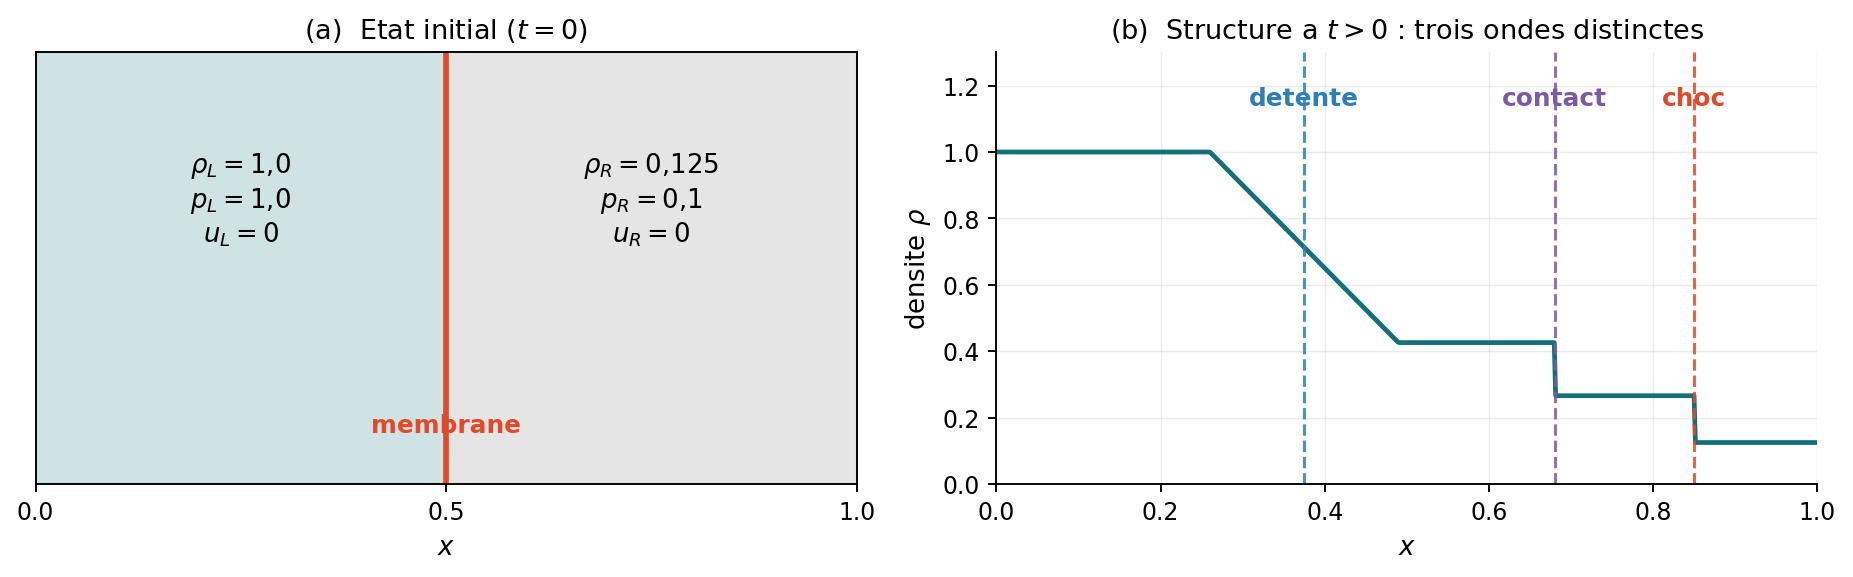
\includegraphics[width=\textwidth]{sod_structure.png}
\caption{Tube à choc de Sod. (a) État initial~: deux états au repos séparés par
une membrane. (b) Structure de la solution à $t>0$~: la rupture engendre
simultanément trois ondes de natures différentes -- une détente régulière, une
discontinuité de contact et un choc.}
\label{fig:sod-struct}
\end{figure}

Sa difficulté tient à ce que la rupture engendre \emph{simultanément trois
ondes de natures différentes} (figure~\ref{fig:sod-struct}b)~:

\begin{itemize}
  \item une \textbf{onde de détente}, régulière et étalée, que le schéma doit
  résoudre avec son ordre élevé~;
  \item une \textbf{discontinuité de contact}, où la densité saute mais où la
  pression et la vitesse restent continues -- c'est l'onde la plus difficile à
  maintenir nette, car rien dans la dynamique ne s'oppose à sa diffusion~;
  \item un \textbf{choc}, discontinuité franche, que le schéma doit capturer
  sans osciller.
\end{itemize}

Un bon schéma doit donc être simultanément précis, non diffusif et non
oscillant, sur trois structures qui appellent des comportements opposés. C'est
précisément parce que Sod est \emph{déjà très bien traité} par TENO5 qu'il
s'est révélé, dans ce projet, le problème le plus résistant à l'amélioration
par apprentissage (section~\ref{sec:volet4}).

\subsection{Problème de Shu--Osher}

Le problème de Shu--Osher est un choc se propageant dans un champ de densité
sinusoïdal. Il combine ainsi, dans un même calcul, une \textbf{discontinuité
forte} et des \textbf{structures fines oscillantes} -- une situation
représentative de l'interaction choc/turbulence.

La difficulté ne vient pas du choc lui-même, qui est capturé sans peine, mais
des oscillations de haute fréquence situées juste derrière lui~: un schéma
trop dissipatif les écrase (voir la figure~\ref{fig:shu-osher} au
chapitre~\ref{chap:realisation}). C'est précisément la marge sur laquelle un
schéma appris peut espérer gagner, et c'est bien sur ce problème que la seule
victoire franche du projet sur le système d'Euler a été obtenue.

Ce contraste entre Sod et Shu--Osher -- un problème où le schéma classique est
déjà quasi optimal, un autre où il laisse une marge dissipative -- constitue
l'un des résultats structurants du rapport, et il est analysé en
section~\ref{sec:volet4}.

\section{Travaux connexes}

Trois directions publiées structurent ce travail.

Stevens \& Colonius \cite{stevens2020} entraînent un réseau à \emph{corriger}
la reconstruction de WENO5 plutôt qu'à la produire de zéro~: le réseau part du
résultat du schéma classique et n'apprend que l'écart à lui appliquer.
Biaiser ainsi le réseau vers un point de départ déjà bon a été, selon les
auteurs, le changement qui a rendu l'entraînement stable. C'est un
raisonnement que ce projet réutilise directement, à deux reprises~: pour le
pré-entraînement par imitation (section~\ref{sec:volet3}) et pour le mécanisme
de mélange convexe (section~\ref{sec:volet4}).

Fu, Hu \& Adams \cite{fu2016} introduisent le schéma TENO, dont ce stage
cherche à améliorer la décision de sélection.

Li, Fu \& Adams \cite{li2022} proposent NENO6, qui entraîne un réseau
\emph{classifieur} prédisant une probabilité « à problème / à garder » par
candidat. Son architecture est celle que reprend le classifieur NN-TENO5 de ce
stage.

\section{Périmètre, missions et méthodologie}

Le sujet, tel qu'énoncé sur la fiche technique du stage, était \emph{« Machine
learning-based numerical scheme for CFD »}, avec trois missions~: une revue de
littérature, la construction d'un réseau de neurones calculant les fonctions de
pondération d'un schéma de type WENO, et l'évaluation de ses performances.

Le périmètre a été volontairement restreint aux problèmes
\textbf{unidimensionnels} (advection linéaire, équation de Burgers, système
d'Euler) et aux schémas d'ordre cinq (WENO5, TENO5). Les extensions
multidimensionnelles et les ordres supérieurs (WENO3/WENO7, TENO3/TENO7) ont
été écartés faute de temps, et sont discutés comme perspectives.

Le travail s'appuie sur un code source existant en accès libre implémentant
l'article WENO5-NN. Plutôt que de repartir de zéro, il l'étend à TENO5, en
reproduit d'abord les résultats publiés comme référence, puis teste une
méthodologie d'entraînement absente des travaux publiés.

\subsection*{Méthodologie de travail}

Le sujet étant une question de recherche plutôt qu'un cahier des charges figé,
le travail a été organisé comme une \textbf{séquence d'expériences
falsifiables} plutôt que comme un plan d'implémentation linéaire~: chaque phase
propose un mécanisme précis, le teste contre la solution vraie, et le conserve,
le corrige ou l'abandonne selon le résultat mesuré.

Deux critères d'évaluation ont été appliqués uniformément à toutes les
expériences~:

\begin{itemize}
  \item \texttt{beats\_teacher}~: l'erreur du réseau contre la solution vraie
  est strictement inférieure à celle du schéma classique contre cette même
  solution. \textbf{C'est le seul critère utilisé pour revendiquer une victoire
  dans ce rapport.}
  \item \texttt{teacher\_fidelity}~: l'erreur du réseau est à moins de $2\%$ de
  celle du schéma classique. Ce critère plus permissif n'a servi qu'à des tests
  d'acceptation précoces et n'est jamais utilisé comme preuve de supériorité.
\end{itemize}

Chaque expérience a été mesurée sur des benchmarks canoniques (hors données
d'entraînement) et documentée immédiatement, y compris lorsqu'elle dégradait
les résultats. C'est pourquoi le journal d'expériences interne du projet
recense 21~phases plutôt qu'une poignée de succès sélectionnés~: plusieurs
correctifs corrects sur le papier se sont révélés mesurablement nuisibles et
ont dû être annulés. Une seconde règle méthodologique, adoptée après la perte
d'un point de sauvegarde fonctionnel, a été de committer et sauvegarder chaque
bon résultat vérifié avant d'entamer l'expérience suivante.

Le tableau~\ref{tab:techno} récapitule l'environnement technique utilisé.

\begin{table}[H]
\centering
\begin{tabularx}{\textwidth}{@{}lX@{}}
\toprule
\textbf{Catégorie} & \textbf{Outils} \\
\midrule
Langage & Python 3 \\
\rowrule
Calcul numérique & NumPy, SciPy \\
\rowrule
Apprentissage (phase 1) & TensorFlow / Keras \\
\rowrule
Apprentissage différentiable (phase 2) & JAX, Optax \\
\rowrule
Visualisation & Matplotlib \\
\rowrule
Gestion de version & Git \\
\rowrule
Rédaction & \LaTeX{} (XeLaTeX) \\
\bottomrule
\end{tabularx}
\caption{Environnement technique du projet.}
\label{tab:techno}
\end{table}

% ============================================================
\chapter{Conception de la solution}
\label{chap:conception}

\section{Architecture générale du code}

Le projet est organisé en modules séparant strictement les schémas numériques,
les réseaux, et la couche différentiable~:

\begin{itemize}
  \item \texttt{src/schemes/} -- implémentations NumPy déterministes de WENO5 et
  TENO5, servant à la fois de schémas de référence et d'enseignants pour
  l'entraînement par imitation.
  \item \texttt{src/networks/} -- définitions des réseaux (Keras) et fonctions
  d'entraînement par imitation.
  \item \texttt{src/core/} -- solveur~: intégration temporelle, séparation de
  flux, conditions aux limites.
  \item \texttt{src/differentiable/} -- réécriture JAX complète et
  différentiable du cœur numérique (section~\ref{sec:jax}).
  \item \texttt{scripts/} -- scripts d'entraînement, d'évaluation et de
  génération de figures.
\end{itemize}

\section{Architecture du réseau classifieur}
\label{sec:archi-reseau}

Le réseau NN-TENO5 est un perceptron multicouche à cinq couches de poids,
suivant l'architecture de NENO6 \cite{li2022}~: un stencil normalisé à
5~valeurs en entrée, quatre couches cachées ReLU de largeur décroissante
(64, 32, 16, 8), et une couche sigmoïde produisant une probabilité de trouble
par candidat de TENO5. La figure~\ref{fig:archi} en donne la structure
détaillée.

\begin{figure}[H]
\centering
\resizebox{\textwidth}{!}{%
\begin{tikzpicture}[
  every node/.style={font=\small},
  iobox/.style={draw, thick, minimum width=0.75cm, minimum height=0.5cm, inner sep=1pt},
  bigbox/.style={draw, thick, minimum width=1.5cm, minimum height=1.3cm},
  smallbox/.style={draw, thick, minimum width=0.9cm, minimum height=0.6cm},
  stripe/.style={draw, thin, minimum width=0.5cm, minimum height=0.28cm, inner sep=0pt},
]
\foreach \i/\lab/\y in {1/u_{i-2}/1.1, 2/u_{i-1}/0.55, 3/u_i/0, 4/u_{i+1}/-0.55, 5/u_{i+2}/-1.1}{
  \node[iobox] (in\i) at (0,\y) {$\lab$};
}
\node at (0,1.75) {$X^0$};
\node[bigbox] (h1) at (2.3,0) {$W^1 \oplus b^1$};
\node at (2.3,-1.0) {\footnotesize 64 neurones};
\node at (2.3,1.0) {\footnotesize $Y^1{=}W^1X^0{+}b^1$};
\foreach \i in {1,...,5}{ \draw[-latex] (in\i.east) -- (h1.west); }
\node[smallbox] (relu1) at (4.0,0) {$\sigma^{\text{RELU}}$};
\draw[-latex] (h1.east) -- (relu1.west);
\foreach \k/\y in {1/1.5,2/1.15,3/0.8,4/0.45,5/0.1,6/-0.25,7/-0.6,8/-0.95,9/-1.3}{
  \node[stripe] (x1-\k) at (5.4,\y) {};
}
\node at (5.4,1.9) {$X^1$};
\draw[-latex] (relu1.east) -- (x1-1.west);
\draw[-latex] (relu1.east) -- (x1-9.west);
\node at (6.6,0) {\Large $\cdots$};
\foreach \k/\y in {1/1.1,2/0.75,3/0.4,4/0.05,5/-0.3,6/-0.65,7/-1.0}{
  \node[stripe] (x4-\k) at (7.8,\y) {};
}
\node at (7.8,1.5) {$X^4$};
\node[bigbox] (h5) at (9.9,0) {$W^5 \oplus b^5$};
\node at (9.9,-1.0) {\footnotesize 3 neurones};
\node at (9.9,1.0) {\footnotesize $Y^5{=}W^5X^4{+}b^5$};
\draw[-latex] (x4-1.east) -- (h5.west);
\draw[-latex] (x4-7.east) -- (h5.west);
\node[smallbox] (sig) at (11.6,0) {$\sigma^{\text{sig}}$};
\draw[-latex] (h5.east) -- (sig.west);
\foreach \i/\lab/\y in {1/p^1/0.6,2/p^2/0,3/p^3/-0.6}{
  \node[iobox] (out\i) at (13.0,\y) {$\lab$};
  \draw[-latex] (sig.east) -- (out\i.west);
}
\node at (13.0,1.2) {$Y^{\text{out}}$};
\node at (0,-2.1) {Couche d'entrée};
\node at (3.15,-2.1) {Couche cachée 1};
\node at (7.2,-2.1) {Couches cachées 2,3,4};
\node at (11.3,-2.1) {Couche de sortie};
\end{tikzpicture}}
\caption{Architecture du classifieur NN-TENO5~: un stencil normalisé à
5~valeurs $X^0$ alimente quatre couches cachées ReLU de largeur décroissante
(64, 32, 16, 8~neurones) puis une couche sigmoïde, produisant une probabilité
de trouble $p^k$ par candidat de TENO5.}
\label{fig:archi}
\end{figure}

Chaque couche $l$ calcule l'application affine $X^{l-1} \to Y^l = W^l X^{l-1} +
b^l$, suivie d'une activation~:
\[
\sigma^{\text{RELU}}(x) = \max(x, 0), \qquad
\sigma^{\text{sig}}(x) = \frac{1}{1+e^{-x}}.
\]
La sortie $[p^1,p^2,p^3]$ se lit comme la probabilité que chaque candidat soit
traversé par une discontinuité. À l'inférence, un candidat est écarté dès que
sa probabilité dépasse $0{,}5$~; pendant l'entraînement par perte déroulée, ce
seuil dur est remplacé par la probabilité continue elle-même, afin que les
gradients puissent traverser la décision.

\section{La fonction de perte physique déroulée}
\label{sec:perte}

L'entraînement par imitation présente une limite structurelle~: sa fonction de
perte ne mesure que la distance à la décision de \emph{l'enseignant}, jamais la
distance à la solution \emph{vraie}. Un réseau ne peut être poussé vers une
réponse qu'on ne lui montre jamais.

L'encadrant a proposé une alternative, la \textbf{fonction de perte physique
déroulée}~: au lieu d'une étiquette d'imitation ponctuelle, le réseau est
utilisé pour avancer réellement la simulation sur $K$ pas de temps, et la
perte est calculée directement contre la solution vraie $K$ pas plus tard.
Elle combine plusieurs termes, dont les trois principaux sont~:
\[
\mathcal{L}_{\text{total}} = \lambda_1\mathcal{L}_{\text{MSE}}
+ \lambda_2\mathcal{L}_{\text{TV}}
+ \lambda_3\mathcal{L}_{\text{Reg}} + \dots
\]
\[
\mathcal{L}_{\text{MSE}} = \frac{1}{N}\sum_{i=1}^{N}\left(u_i^{n+K} - u_{i,\text{exact}}^{n+K}\right)^2,
\qquad
\mathcal{L}_{\text{TV}} = \max\left(0,\ \mathrm{TV}(u^{n+K}) - \mathrm{TV}(u^{n})\right).
\]
Le premier, $\mathcal{L}_{\text{MSE}}$, mesure l'écart à la solution vraie
après $K$ pas -- c'est le terme central, celui qui rend l'approche différente
de l'imitation. Le deuxième pénalise toute augmentation de la variation totale
$\mathrm{TV}(v) = \sum_i |v_{i+1}-v_i|$, c'est-à-dire toute apparition
d'oscillations parasites. Le troisième, $\mathcal{L}_{\text{Reg}}$, ancre la
solution du réseau sur celle du schéma classique et l'empêche de s'en écarter
arbitrairement. S'y ajoute un terme de cohérence entre cellules voisines
(principe \emph{Boundary Variation Diminishing}, ou BVD~\cite{fu2016})~: à une
interface donnée, la cellule de gauche et celle de droite proposent chacune
une valeur, et ce terme pénalise leur désaccord. Enfin, pour le système
d'Euler, un dernier terme pénalise les états non physiques -- densité ou
pression négatives (section~\ref{sec:instabilite}).

\section{La réécriture différentiable en JAX}
\label{sec:jax}

Cette formulation ne pouvait pas être testée dans le code d'origine~: dérouler
$K$ pas de simulation exige que \emph{toute} la chaîne -- reconstruction,
séparation de flux, intégration temporelle, projection caractéristique -- soit
différentiable de bout en bout. Or le solveur NumPy ne porte aucun gradient, et
\texttt{model.predict()} de Keras se détache entièrement du graphe.

Le module \texttt{src/differentiable/} est donc une réécriture JAX complète du
cœur numérique, et non une simple enveloppe. Le tableau~\ref{tab:jax} résume
les composants réimplémentés.

\begin{table}[H]
\centering
\begin{tabularx}{\textwidth}{@{}lX@{}}
\toprule
\textbf{Composant} & \textbf{Contenu réimplémenté en JAX} \\
\midrule
Reconstruction & TENO5 complet~: $\beta_k$, $\tau_5$, seuillage, renormalisation \\
\rowrule
Solveur & SSPRK3, séparation de Lax--Friedrichs, conditions aux limites \\
\rowrule
Euler & base propre de Roe, projection caractéristique, réparation de positivité \\
\rowrule
Réseau & propagation avant du MLP, sans dépendance à Keras \\
\rowrule
Perte & les cinq termes, dont la pénalité de positivité d'Euler \\
\bottomrule
\end{tabularx}
\caption{Composants réécrits dans le module différentiable JAX.}
\label{tab:jax}
\end{table}

Le seuillage binaire de TENO5 pose ici une difficulté spécifique~: la fonction
$\delta_k$ a une dérivée nulle presque partout, ce qui bloquerait toute
rétropropagation. C'est pourquoi la probabilité continue du réseau remplace le
seuil dur pendant l'entraînement.

% ============================================================
\chapter{Réalisation et expérimentations}
\label{chap:realisation}

\section{Volet 1~: WENO5-NN vs.\ WENO5}
\label{sec:volet1}

Le premier volet reproduit les trois configurations publiées par Stevens \&
Colonius \cite{stevens2020}, à partir de leur jeu d'entraînement d'origine
(75\,241 échantillons), afin d'établir une référence vérifiée.

\textbf{Advection d'un créneau.} WENO5-NN réduit l'erreur $L_1$ de $28{,}7\%$,
$L_2$ de $17{,}1\%$, $L_\infty$ de $5{,}2\%$ et la largeur de choc de
$21{,}4\%$ face à WENO5~: le résultat le plus net des trois cas.
La figure~\ref{fig:step-width} explique ce gain~: la largeur de la
discontinuité produite par WENO5 croît continûment sous l'effet de la
diffusion numérique, tandis que celle du réseau se stabilise.

\begin{figure}[H]
\centering
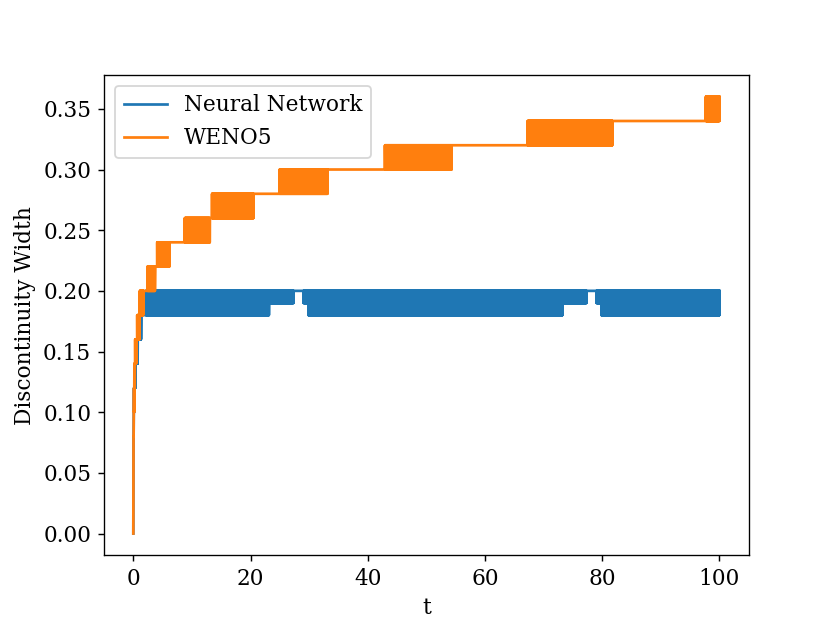
\includegraphics[width=0.60\textwidth]{step_advection/discontinuity_width_vs_time.png}
\caption{Largeur de discontinuité en fonction du temps. Celle de WENO5 croît de
façon monotone sous l'effet de la diffusion numérique~; celle du réseau se
stabilise autour de $0{,}19$, ce qui explique le gain de $21{,}4\%$ mesuré à
$t=100$.}
\label{fig:step-width}
\end{figure}

\textbf{Équation de Burgers.} Résultat franchement mitigé~: le réseau gagne à
3~des 4~résolutions testées et perd à la quatrième
(figure~\ref{fig:burgers-grid}). Cela rejoint l'observation des auteurs
eux-mêmes~: les deux schémas se comportent de façon similaire pour un vrai
choc, l'avantage du réseau venant surtout de la région lisse pré-choc.

\begin{figure}[H]
\centering
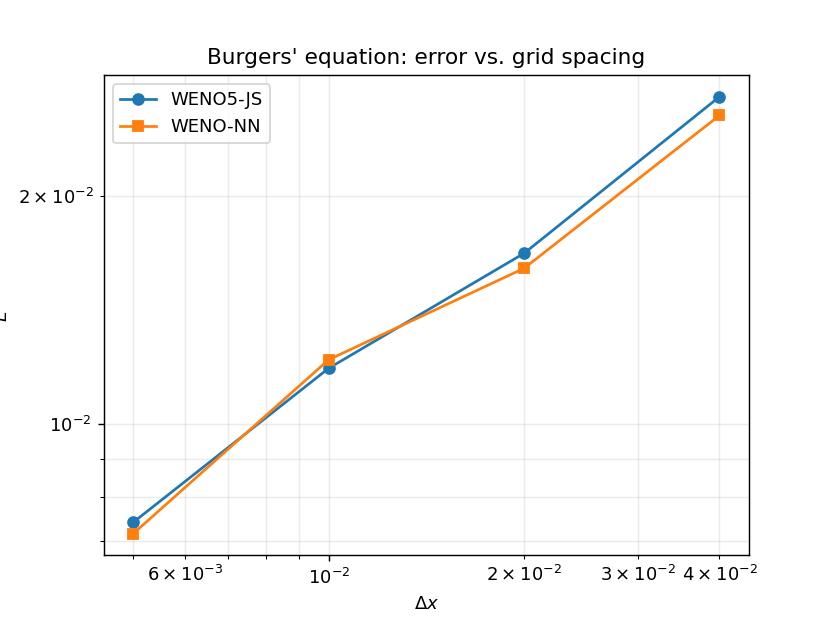
\includegraphics[width=0.56\textwidth]{burgers/error_vs_grid_spacing.png}
\caption{Équation de Burgers~: erreur $L_2$ en fonction du pas d'espace. Le
réseau (orange) passe sous WENO5-JS (bleu) à trois résolutions sur quatre, et
repasse légèrement au-dessus autour de $\Delta x \approx 10^{-2}$.}
\label{fig:burgers-grid}
\end{figure}

\textbf{Sod et Shu--Osher.} Quasi-égalité~: les courbes sont visuellement
indiscernables de la solution exacte. C'est néanmoins une défaite sous le
critère strict, l'erreur $L_\infty$ du réseau étant supérieure de $0{,}265\%$
pour Sod et $0{,}551\%$ pour Shu--Osher.

Le verdict du volet~1 est donc une \textbf{égalité fortement dépendante du
problème}~: une victoire nette là où la distribution d'entraînement du réseau
correspond bien au problème, et une quasi-égalité défavorable sur les cas qui
la sollicitent davantage.

\section{Volet 2~: NN-TENO5 par imitation vs.\ TENO5}
\label{sec:volet2}

Le deuxième volet applique la même idée à TENO5, avec le classifieur décrit en
section~\ref{sec:archi-reseau}, entraîné à reproduire la décision
garder/écarter de TENO5.

Par construction, un réseau entraîné uniquement à imiter un enseignant ne peut
pas dépasser la qualité de reconstruction de celui-ci, sauf par son propre
bruit de généralisation. Les mesures le confirment~: sur 3~des 4~benchmarks
scalaires testés, NN-TENO5 produit une égalité \emph{exacte} avec TENO5~; sur
l'advection d'un créneau, il perd de $0{,}64\%$~; sur les benchmarks d'Euler,
il produit deux petites victoires compatibles avec le plafond d'imitation
(reproduire ou perturber très légèrement la décision de l'enseignant peut
occasionnellement tomber plus près de la solution vraie par hasard, sans
amélioration systématique).

Deux tentatives de dépassement à l'intérieur du paradigme d'imitation --
entraînement sur cible exacte, extension à un stencil WENO7 à 7~points,
recherche d'hyperparamètres étendue, et entraînement sur données TENO5
« réétiquetées par oracle » -- ont toutes produit soit un résultat négatif,
soit une petite victoire plafonnant au même niveau. Ce constat, \textbf{le
plafond est structurel au paradigme d'imitation lui-même, non un défaut de
réglage}, a directement motivé la seconde phase du stage.

\section{Volet 3~: benchmarks scalaires par perte déroulée}
\label{sec:volet3}

La perte déroulée a d'abord été testée sur l'advection et Burgers. Trois
obstacles ont dû être levés successivement.

\textbf{Obstacle 1 -- déséquilibre des termes de perte.} Entraîner en suivant
littéralement les équations de la proposition, avec $\mathcal{L}_{\text{TV}}$
et $\mathcal{L}_{\text{Reg}}$ non normalisés, laisse le gradient de
$\mathcal{L}_{\text{TV}}$ dominer celui de $\mathcal{L}_{\text{MSE}}$ d'un
facteur~$\approx 4$, même après application de son poids $0{,}1$. La
figure~\ref{fig:loss-curves} montre le diagnostic et l'effet du correctif
(normalisation en moyenne plutôt qu'en somme).

\begin{figure}[H]
\centering
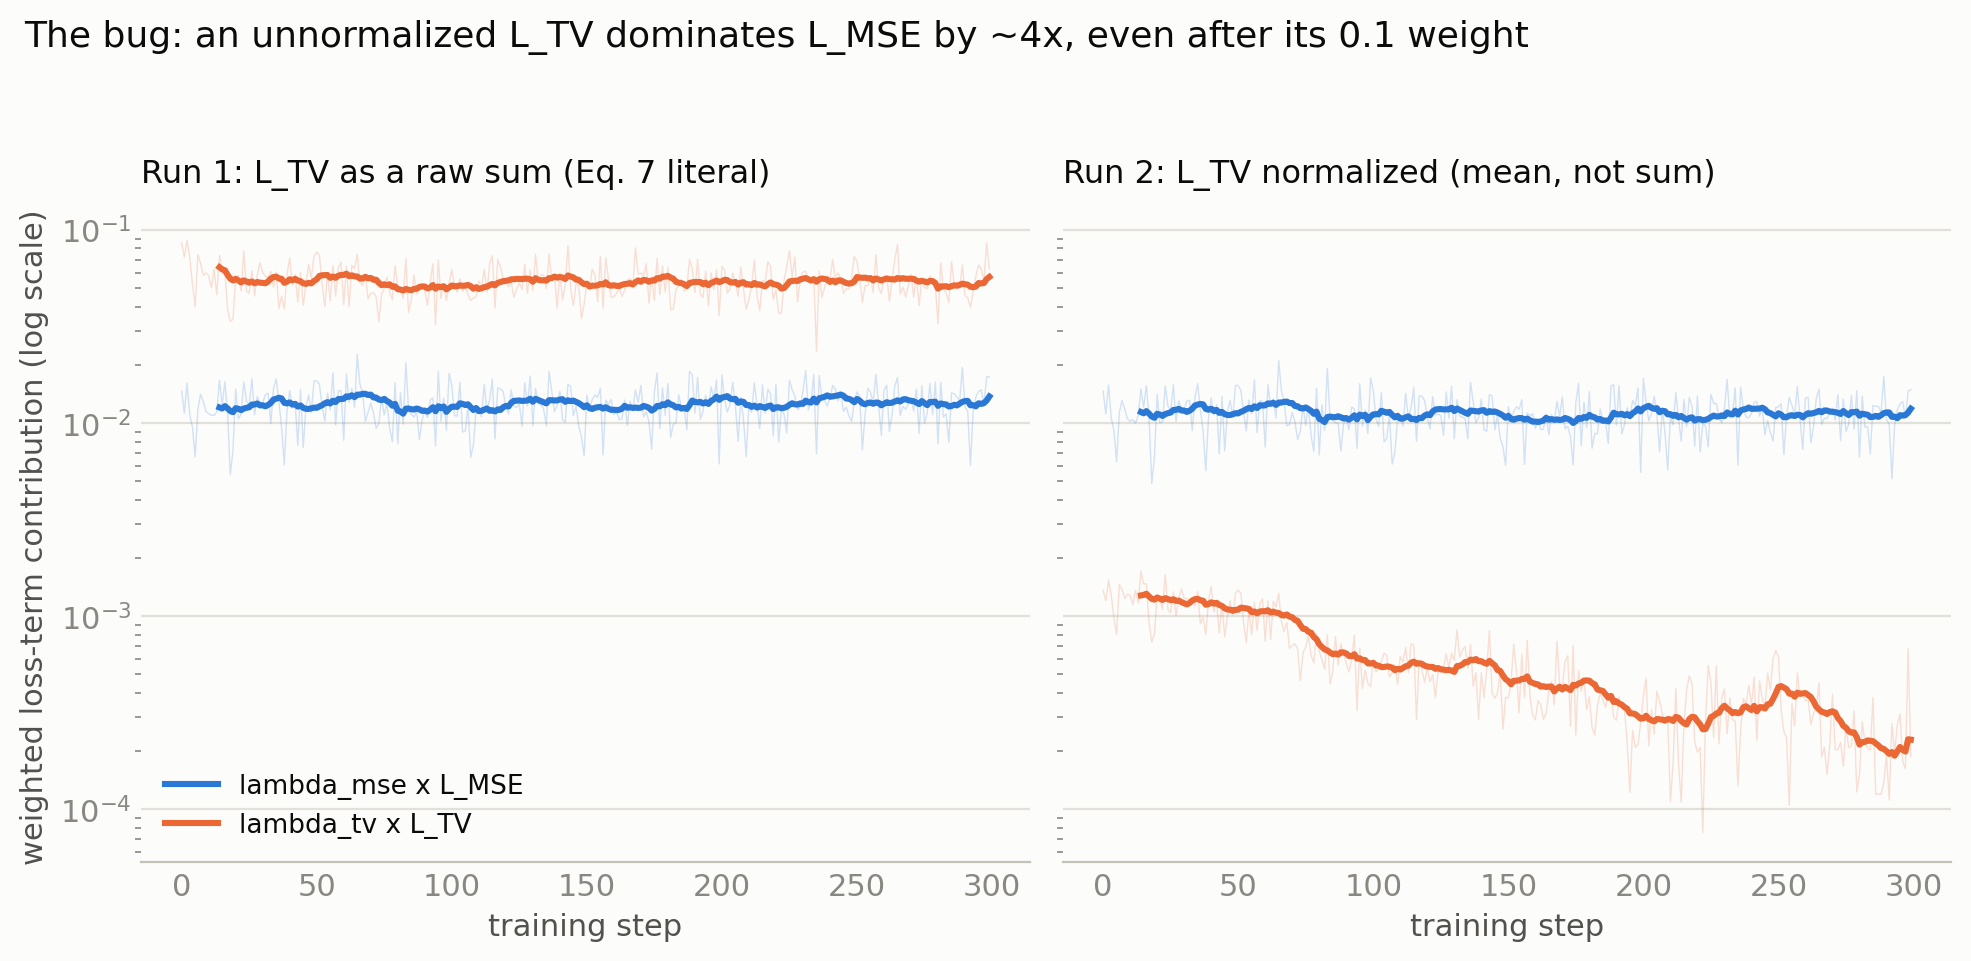
\includegraphics[width=\textwidth]{01_scalar_training_curves.png}
\caption{Contributions pondérées des termes de perte au cours de
l'entraînement. À gauche, $\mathcal{L}_{\text{TV}}$ brut domine
$\mathcal{L}_{\text{MSE}}$ d'environ un facteur~4 et l'entraînement optimise
en réalité la mauvaise quantité~; à droite, après normalisation, l'équilibre
attendu est rétabli et $\mathcal{L}_{\text{TV}}$ décroît.}
\label{fig:loss-curves}
\end{figure}

\textbf{Obstacle 2 -- initialisation.} Entraîner un réseau initialisé
aléatoirement directement contre la perte déroulée échoue complètement. Le
correctif reprend le motif déjà validé au volet~2~: pré-entraînement par
imitation, puis affinage par perte déroulée.

\textbf{Obstacle 3 -- généralisation.} Le réseau obtenu gagnait 2~des 3~tests
tenus à l'écart, mais ne généralisait ni au benchmark canonique à pleine
échelle, ni au flux non linéaire de Burgers, absent de sa distribution
d'entraînement.

Le correctif final réutilise un mécanisme développé d'abord pour le système
d'Euler (section~\ref{sec:volet4})~: une \textbf{tête de mélange} entraînée
séparément, produisant un coefficient de combinaison convexe
$\lambda \in [0,1]$ entre la reconstruction de TENO5 et celle du réseau~:
\[
u_{\text{final}} = (1-\lambda)\, u_{\text{TENO5}} + \lambda\, u_{\text{réseau}},
\]
complété par des exemples d'entraînement à flux de Burgers. Ce mécanisme
garantit que le réseau ne peut qu'interpoler \emph{vers} sa propre
reconstruction depuis celle de TENO5, jamais la dépasser dans la mauvaise
direction.

Deux observations méritent d'être soulignées. D'abord, la tête \emph{non
entraînée} (avec un biais initial conservateur donnant $\lambda \approx
4{,}7\%$ uniformément) gagnait déjà sur les deux benchmarks canoniques
\emph{avant tout entraînement supplémentaire}. Ensuite, et de façon
contre-intuitive, \textbf{le mélange uniforme bat le mélange concentré sur les
stencils à problème}~: laisser le réseau corriger aussi les petites erreurs du
schéma classique en région lisse apporte davantage que de le cantonner aux
zones que le schéma classique signale.

\section{Volet 4~: le système d'Euler}
\label{sec:volet4}

Le système d'Euler est plus difficile pour deux raisons indépendantes~: la
reconstruction y est couplée et caractéristique (section~\ref{sec:fond-vf}), et
la solution doit rester physiquement valide (densité et pression positives) à
\emph{chaque} étape intermédiaire de l'entraînement, pas seulement à
convergence.

\subsection{Diagnostic et correction de l'instabilité}
\label{sec:instabilite}

La première tentative d'entraînement a divergé purement et simplement~: les
valeurs d'état croissaient sans borne en quelques sous-pas SSPRK3, quelle que
soit l'augmentation de la marge de dissipation de la séparation de
Lax--Friedrichs. La figure~\ref{fig:instab} montre le résultat décisif~:
\emph{augmenter} la dissipation fait arriver l'instabilité \emph{plus vite},
ce qui écarte l'hypothèse d'un choc sous-résolu et oriente vers un bogue.

\begin{figure}[H]
\centering
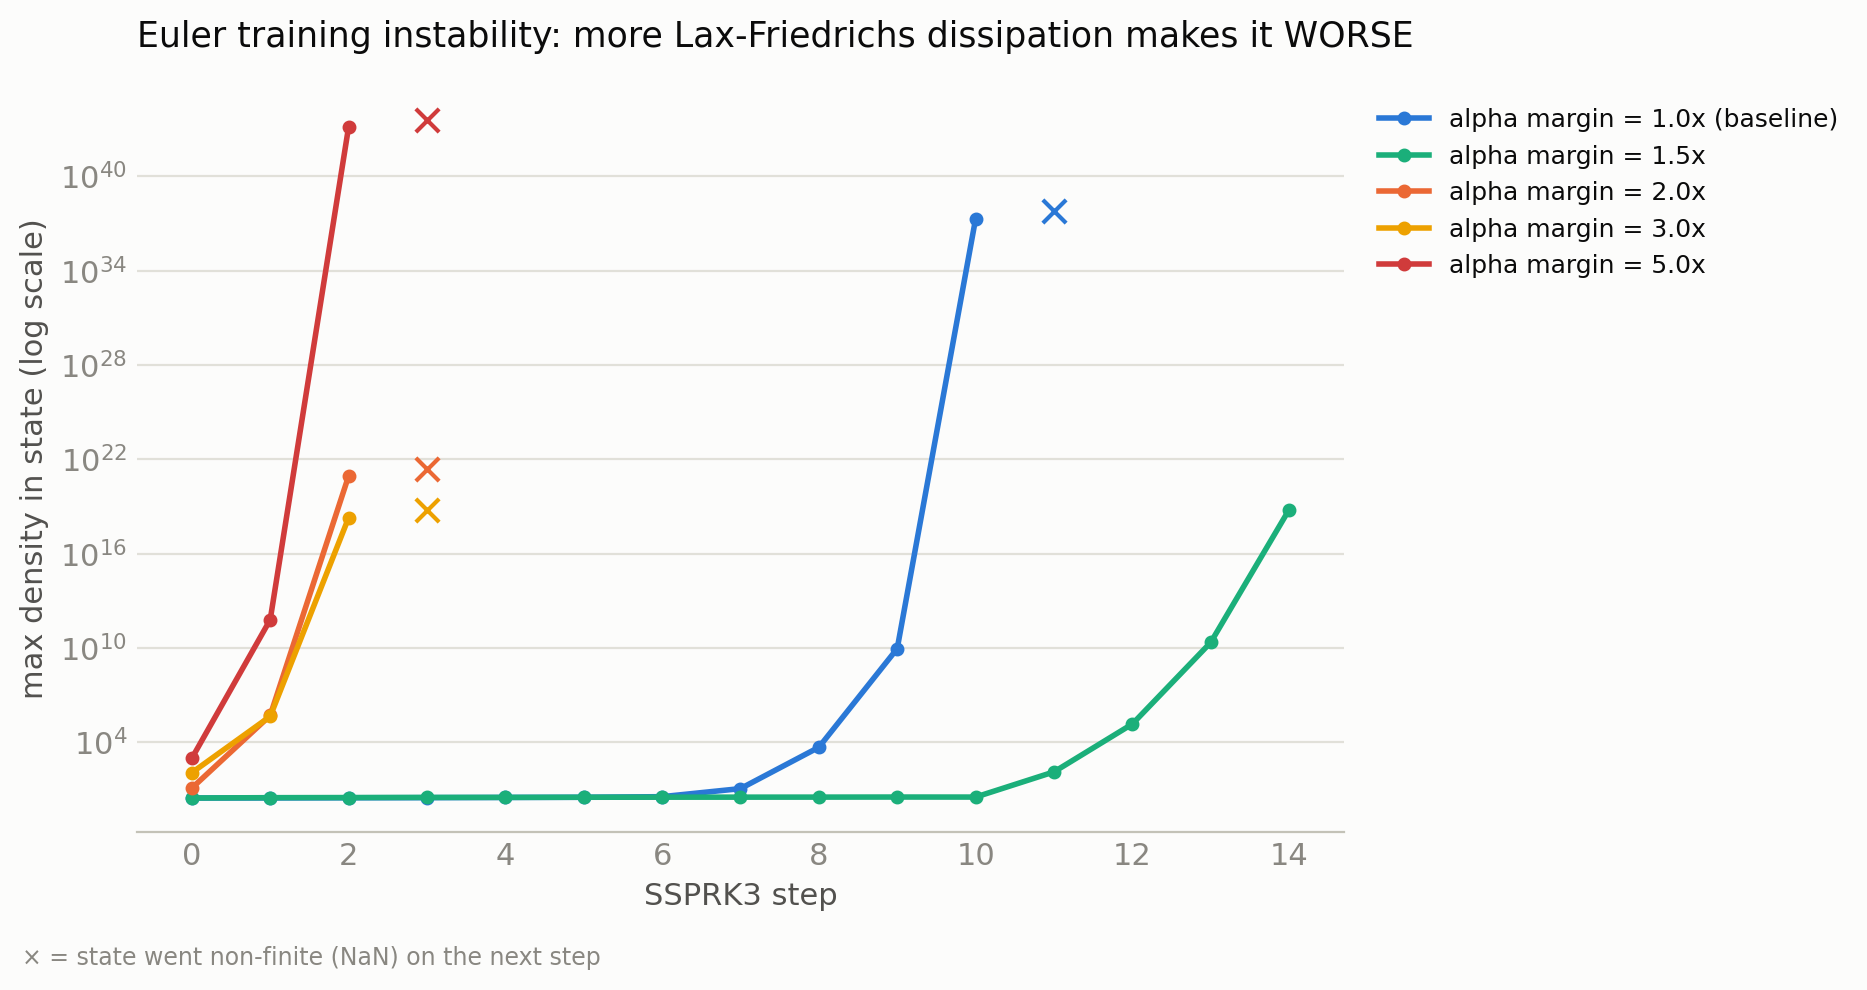
\includegraphics[width=0.72\textwidth]{04_euler_instability.png}
\caption{Instabilité à l'entraînement sur Euler~: la densité maximale diverge
d'autant plus vite que la marge de dissipation est augmentée. Ce comportement
contre-intuitif écarte la dissipation numérique insuffisante comme cause et
oriente le diagnostic vers le traitement des violations de positivité.}
\label{fig:instab}
\end{figure}

Deux défauts concrets ont été identifiés et corrigés~:

\begin{enumerate}
  \item \textbf{Une pénalité de positivité structurellement inerte.} Le terme
  censé pénaliser les états non physiques était calculé sur l'état final
  \emph{déjà réparé} de chaque pas, après application d'un écrêtage~: il ne
  pouvait donc mathématiquement jamais être non nul. Corrigé en calculant la
  pénalité sur les sous-étapes avant réparation.
  \item \textbf{Un mécanisme de réparation incomplet.} La réparation ne testait
  que le signe~; elle ne détectait ni les valeurs non finies
  (\texttt{NaN}/\texttt{Inf}) ni les magnitudes non bornées, qui peuvent naître
  d'une reconstruction imparfaite réinjectée dans la base propre de Roe du pas
  suivant. Corrigé par l'ajout de tests explicites de finitude et de magnitude.
\end{enumerate}

Combinés à la clarification de la définition du terme BVD apportée par
l'encadrant, ces correctifs ont produit le premier entraînement d'Euler qui ne
diverge pas.

\subsection{La tête de mélange dédiée}

Le mécanisme qui a finalement produit une victoire canonique est le mélange
convexe introduit en section~\ref{sec:volet3}, mais son coefficient $\lambda$
devait être calculé par une tête \emph{dédiée}, entraînée séparément, plutôt
que réutilisé depuis la sortie de probabilité de trouble du réseau. Réutiliser
ce signal faisait porter à $\lambda$ deux rôles incompatibles -- signaler un
problème \emph{et} calibrer la confiance accordée au réseau -- et a causé trois
régressions distinctes. Une petite tête entraînée spécifiquement, initialisée
de façon conservatrice (biais $=-3$, soit $\lambda \approx 4{,}7\%$ au départ),
a corrigé ce point et produit la première victoire canonique franche du projet
(figure~\ref{fig:shu-osher}).

\begin{figure}[H]
\centering
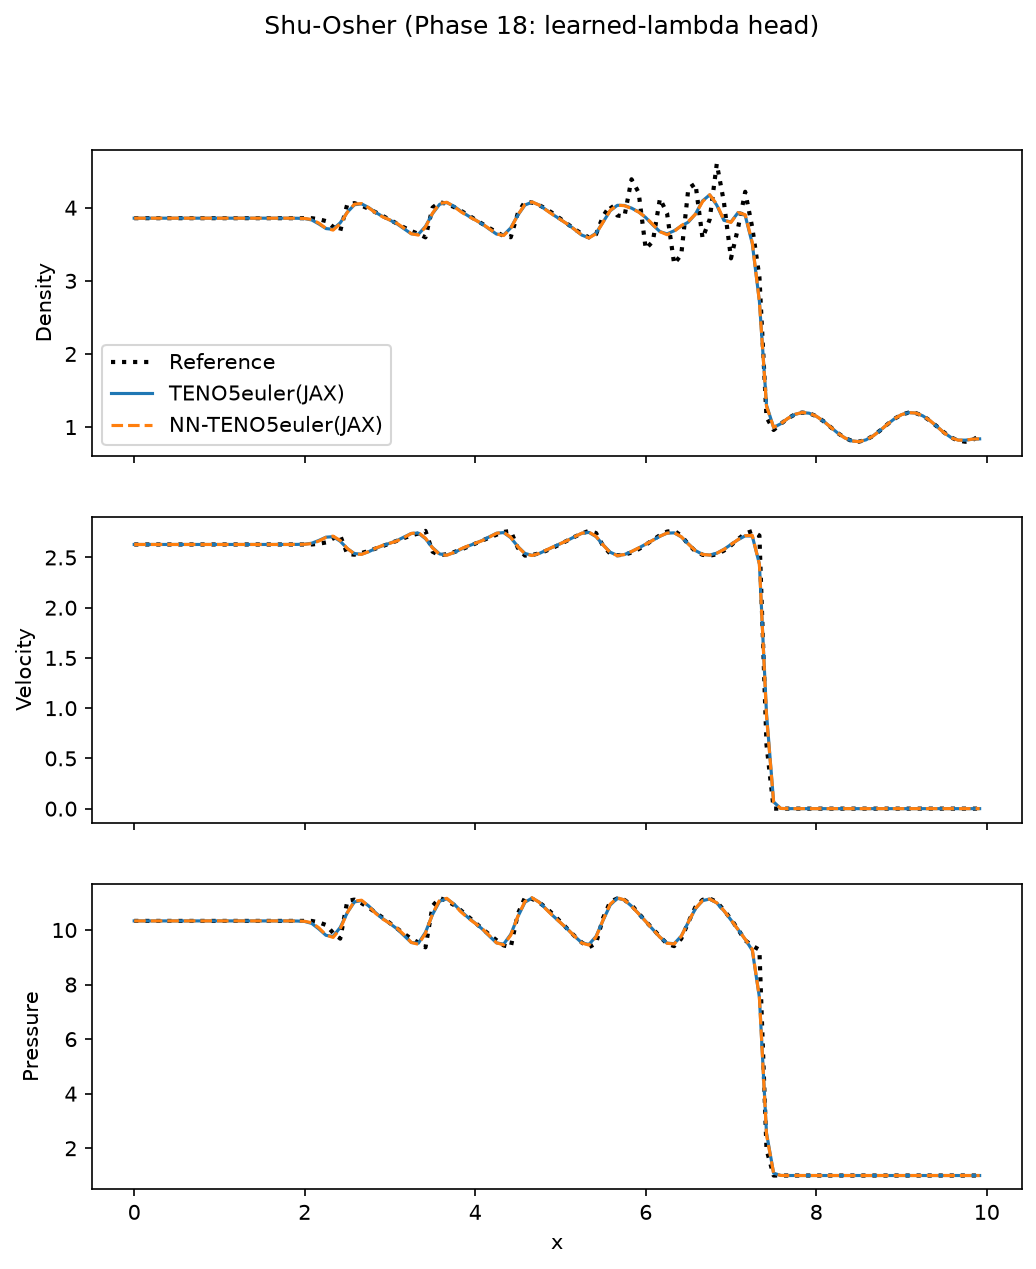
\includegraphics[width=0.56\textwidth]{euler_jax_comparison/shu_osher_phase18.png}
\caption{Shu--Osher avec tête de mélange dédiée~: NN-TENO5euler et TENO5euler
sont visuellement quasi identiques face à la référence, NN-TENO5euler étant
$1{,}84\%$ plus précis en $L_1$ moyen sur les trois variables conservées.}
\label{fig:shu-osher}
\end{figure}

Le cas de Sod, en revanche, est resté une quasi-égalité légèrement défavorable
au réseau même après ce correctif. Deux tentatives
supplémentaires -- un taux d'apprentissage 50~fois plus élevé pour la seule
tête de mélange, et une porte enrichie voyant le stencil brut plutôt que le
seul résumé de probabilité -- n'ont déplacé le ratio de Sod que marginalement
($1{,}0045\times$, puis $1{,}0026\times$), jamais au-delà de la parité.

Un balayage direct d'un coefficient $\lambda$ fixe (non appris) a confirmé
qu'il s'agit d'une \textbf{limite structurelle} du schéma appris sur Sod, et
non d'un défaut de calibrage~: l'erreur de Sod croît de façon
\emph{monotone} avec chaque $\lambda$ testé de $0$ à $0{,}3$, tandis que celle
de Shu--Osher \emph{décroît} de façon monotone jusqu'à $\lambda \approx 0{,}2$
sur le même balayage. Aucun réglage de la porte ne peut corriger un schéma de
base qui est, sur ce problème précis, simplement moins précis que TENO5.

% ============================================================
\chapter{Résultats, analyse critique et limites}
\label{chap:resultats}

\section{Métriques d'évaluation}
\label{sec:metriques}

Tous les résultats sont mesurés avec le même jeu de métriques, appliqué
identiquement au schéma classique et au réseau. Avec $d_i = u_i -
u_i^{\text{ref}}$~:
\[
L_1 = \frac{1}{N}\sum_i |d_i|, \qquad
L_2 = \sqrt{\frac{1}{N}\sum_i d_i^2}, \qquad
L_\infty = \max_i |d_i|.
\]
Pour Euler, elles sont calculées indépendamment par variable conservée
(densité, quantité de mouvement, énergie) puis moyennées en un scalaire
$\bar L_1$. Trois diagnostics complémentaires sont utilisés~: la variation
totale $\mathrm{TV}(u)=\sum_i|u_{i+1}-u_i|$ (dont un excès signale une
oscillation parasite), la positivité ($\min_i \rho_i > 0$ et $\min_i p_i > 0$),
et l'erreur de localisation du choc et du contact.

\section{Résultats consolidés}
\label{sec:consolide}

Les tableaux~\ref{tab:volet3} et~\ref{tab:volet4} consolident les mesures
finales, et le tableau~\ref{tab:synthese} résume les quatre volets.

\begin{table}[H]
\centering
\begin{adjustbox}{max width=\textwidth}
\begin{tabular}{lrrrl}
\toprule
\textbf{Benchmark} & \textbf{TENO5} & \textbf{NN-TENO5 (JAX)} & \textbf{Ratio} & \textbf{Verdict} \\
\midrule
Advection ($L_1$) & 3{,}4819e-02 & 3{,}3813e-02 & $0{,}9711\times$ & \textbf{VICTOIRE} \\
\rowrule
Advection ($L_2$) & 9{,}8960e-02 & 9{,}5521e-02 & $0{,}9653\times$ & \textbf{VICTOIRE} \\
\rowrule
Burgers ($L_1$, hors distribution) & 2{,}0697e-04 & 1{,}7873e-04 & $0{,}8636\times$ & \textbf{VICTOIRE} \\
\rowrule
Burgers ($L_2$, hors distribution) & 8{,}1670e-04 & 6{,}6493e-04 & $0{,}8142\times$ & \textbf{VICTOIRE} \\
\bottomrule
\end{tabular}
\end{adjustbox}
\caption{Volet~3 (scalaire), évaluation à l'échelle canonique. NN-TENO5 gagne
sur les deux benchmarks, y compris Burgers, explicitement hors distribution
d'entraînement.}
\label{tab:volet3}
\end{table}

\begin{table}[H]
\centering
\begin{adjustbox}{max width=\textwidth}
\begin{tabular}{lrrrl}
\toprule
\textbf{Benchmark} & \textbf{TENO5euler $\bar L_1$} & \textbf{NN-TENO5euler $\bar L_1$} & \textbf{Ratio} & \textbf{Verdict} \\
\midrule
Sod & 8{,}2583e-03 & 8{,}2871e-03 & $1{,}0035\times$ & DÉFAITE \\
\rowrule
Shu--Osher & 2{,}1319e-01 & 2{,}0926e-01 & $0{,}9816\times$ & \textbf{VICTOIRE} \\
\bottomrule
\end{tabular}
\end{adjustbox}
\caption{Volet~4 (Euler), meilleur modèle obtenu (tête de mélange dédiée). Sod
est $0{,}35\%$ moins précis~; Shu--Osher est $1{,}84\%$ plus précis -- première
victoire franche contre un schéma classique sur un benchmark canonique obtenue
dans ce projet.}
\label{tab:volet4}
\end{table}

\begin{table}[H]
\centering
\small
\begin{tabularx}{\textwidth}{@{}>{\raggedright\arraybackslash}p{0.20\textwidth}>{\raggedright\arraybackslash}p{0.20\textwidth}>{\centering\arraybackslash}p{0.10\textwidth}>{\raggedright\arraybackslash}X@{}}
\toprule
\textbf{Volet} & \textbf{Verdict} & \textbf{Résultat} & \textbf{Observation principale} \\
\midrule
1. WENO5-NN vs.\ WENO5 & Fortement dépendant du problème & ÉGALITÉ & Victoire sur l'advection et 3/4 résolutions de Burgers~; légère défaite sur Sod et Shu--Osher. \\
\rowrule
2. NN-TENO5 (imitation) & Reproduit son enseignant & ÉGALITÉ & Trois égalités exactes, deux petites victoires Euler, une défaite sur l'advection. \\
\rowrule
3. NN-TENO5 (perte déroulée), scalaire & Victoire sur les deux benchmarks & \textbf{VICTOIRE} & $3{,}5\%$ sur l'advection, $18{,}6\%$ sur Burgers (hors distribution). \\
\rowrule
4. NN-TENO5euler (perte déroulée) & Première victoire canonique & \textbf{VICTOIRE} & $1{,}84\%$ sur Shu--Osher~; Sod reste une quasi-égalité structurelle. \\
\bottomrule
\end{tabularx}
\caption{Synthèse globale des quatre volets.}
\label{tab:synthese}
\end{table}

\section{Analyse critique}

Deux résultats se dégagent, et ce sont les deux faces d'une même observation~:
\textbf{la manière dont un réseau est entraîné compte davantage que son
architecture}.

Le premier est le plafond d'imitation du volet~2. Un réseau entraîné à copier
un enseignant hérite de ses limites~; aucune quantité de réglage
d'hyperparamètres, d'élargissement du stencil ou de réétiquetage n'a permis de
le franchir. Le second est le succès des volets~3 et~4~: en changeant le
\emph{signal} d'entraînement -- une perte mesurée contre la solution vraie
après $K$ pas réels, plutôt que contre la décision d'un enseignant -- le même
type de réseau devient capable de dépasser le schéma classique, y compris sur
un flux absent de sa distribution d'entraînement.

Trois réserves doivent cependant accompagner ces résultats.

\textbf{Les gains sont modestes et non uniformes.} $1{,}84\%$ sur Shu--Osher est
une victoire réelle mais faible, et Sod reste défavorable. Le balayage de
$\lambda$ montre que le comportement est de signe opposé sur les deux
problèmes, ce qui suggère que le schéma appris n'améliore pas la reconstruction
de façon universelle, mais seulement sur certaines structures d'écoulement.

\textbf{Le coût de calcul n'est pas compensé.} Chaque variante neuronale
s'exécute nettement plus lentement par cellule que son équivalent classique --
environ $5$ à $18\times$ pour les modèles fondés sur Keras. Les gains de
précision rapportés ne constituent donc pas, en l'état, un avantage
calcul/précision.

\textbf{Le mécanisme gagnant est un garde-fou.} La tête de mélange convexe
garantit que le réseau ne peut qu'interpoler vers sa propre reconstruction sans
la dépasser. C'est ce qui rend le résultat robuste, mais cela borne aussi
mécaniquement l'amélioration atteignable.

\section{Limites et perspectives}

Le travail est resté limité aux problèmes unidimensionnels, scalaires et
d'Euler, et aux schémas d'ordre cinq. Trois prolongements naturels se dégagent~:

\begin{itemize}
  \item \textbf{Extension à WENO7/TENO7 et à la 2D.} La pile différentiable et
  le mécanisme de mélange convexe sont indépendants de l'ordre et de la
  dimension~; leur extension est essentiellement un travail d'ingénierie.
  \item \textbf{Réduction du coût d'inférence.} Le surcoût actuel vient d'une
  implémentation non optimisée~; une distillation vers un réseau plus petit, ou
  une compilation dédiée, sont des pistes directes.
  \item \textbf{Compréhension de l'asymétrie Sod / Shu--Osher.} Identifier
  quelle caractéristique de l'écoulement rend le mélange bénéfique dans un cas
  et nuisible dans l'autre serait le prolongement scientifiquement le plus
  utile, et permettrait peut-être de conditionner $\lambda$ sur cette
  caractéristique.
\end{itemize}

% ============================================================
\chapter*{Conclusion}
\addcontentsline{toc}{chapter}{Conclusion}
\markboth{Conclusion}{}

Ce stage avait pour objectif de déterminer si un réseau de neurones peut
améliorer un schéma numérique classique de capture de chocs, mesuré strictement
contre la solution vraie. La réponse obtenue est nuancée mais positive, et elle
tient surtout à \emph{la façon} dont le réseau est entraîné.

Les deux premiers volets, fondés sur l'entraînement par imitation, aboutissent à
une égalité~: reproduire les résultats publiés de WENO5-NN confirme leur
caractère fortement dépendant du problème, et étendre l'approche à TENO5 met en
évidence un plafond structurel -- un réseau qui copie un enseignant ne peut pas
le dépasser. Ce résultat négatif a été le point de bascule du stage.

Les deux volets suivants, fondés sur la fonction de perte physique déroulée
proposée par l'encadrant, franchissent ce plafond. Ils ont exigé une réécriture
complète et différentiable du cœur numérique en JAX, sans laquelle la
proposition n'était pas testable. Ils aboutissent à des victoires vérifiées sur
les benchmarks canoniques scalaires ($3{,}5\%$ sur l'advection, $18{,}6\%$ sur
Burgers hors distribution) et à une première victoire franche sur le système
d'Euler ($1{,}84\%$ sur Shu--Osher), obtenue via une tête de mélange convexe
dédiée. Le cas de Sod reste défavorable, et un balayage direct du coefficient de
mélange établit qu'il s'agit d'une limite structurelle du schéma appris.

Sur le plan personnel, ce stage a été formateur d'abord par sa discipline
expérimentale. Les résultats les plus utiles n'ont pas été les victoires, mais
les diagnostics~: comprendre pourquoi augmenter la dissipation aggravait
l'instabilité a mené à un terme de perte structurellement inerte~; comprendre
pourquoi le réseau plafonnait a mené au changement de paradigme d'entraînement.
J'ai aussi appris à traiter un résultat négatif comme une donnée à documenter
plutôt que comme un échec à masquer -- c'est ce qui a rendu la progression
mesurable, et c'est la compétence que je retire le plus nettement de ces deux
mois.

% ============================================================
\begin{thebibliography}{9}
\addcontentsline{toc}{chapter}{Références bibliographiques}

\bibitem{harten1987}
A.~Harten, B.~Engquist, S.~Osher, S.~R.~Chakravarthy.
\emph{Uniformly high order accurate essentially non-oscillatory schemes,~III}.
Journal of Computational Physics, 71(2):231--303, 1987.

\bibitem{shu1988}
C.-W.~Shu, S.~Osher.
\emph{Efficient implementation of essentially non-oscillatory shock-capturing
schemes}.
Journal of Computational Physics, 77(2):439--471, 1988.

\bibitem{jiang1996}
G.-S.~Jiang, C.-W.~Shu.
\emph{Efficient implementation of weighted ENO schemes}.
Journal of Computational Physics, 126(1):202--228, 1996.

\bibitem{borges2008}
R.~Borges, M.~Carmona, B.~Costa, W.~S.~Don.
\emph{An improved weighted essentially non-oscillatory scheme for hyperbolic
conservation laws}.
Journal of Computational Physics, 227(6):3191--3211, 2008.

\bibitem{fu2016}
L.~Fu, X.~Y.~Hu, N.~A.~Adams.
\emph{A family of high-order targeted ENO schemes for compressible-fluid
simulations}.
Journal of Computational Physics, 305:333--359, 2016.

\bibitem{stevens2020}
B.~Stevens, T.~Colonius.
\emph{Enhancement of shock-capturing methods via machine learning}.
Theoretical and Computational Fluid Dynamics, 34:483--496, 2020.

\bibitem{li2022}
Y.~Li, L.~Fu, N.~A.~Adams.
\emph{A six-point neuron-based ENO (NENO6) scheme for compressible fluid
dynamics}.
arXiv:2207.08500, 2022.

\bibitem{wen2020}
X.~Wen, W.~S.~Don, Z.~Gao, J.~S.~Hesthaven.
\emph{An edge detector based on artificial neural network with application to
hybrid Compact-WENO finite difference scheme}.
Journal of Scientific Computing, 83(49), 2020.

\bibitem{sod1978}
G.~A.~Sod.
\emph{A survey of several finite difference methods for systems of nonlinear
hyperbolic conservation laws}.
Journal of Computational Physics, 27(1):1--31, 1978.

\bibitem{jax2018}
J.~Bradbury, R.~Frostig, P.~Hawkins, et al.
\emph{JAX: composable transformations of Python+NumPy programs}.
\url{http://github.com/google/jax}, 2018.

\bibitem{nasa1993}
L.~Weinstein / NASA.
\emph{Schlieren photograph of T-38 shock waves} (Mach~1,1, 13\,000~pieds).
NASA Dryden Flight Research Center Photo Collection, photo EC94-42528-1,
13~décembre 1993. Domaine public (œuvre du gouvernement des États-Unis).
Disponible sur Wikimedia Commons~:
\url{https://commons.wikimedia.org/wiki/File:Schlieren_photograph_of_T-38_shock_waves.jpg}

\end{thebibliography}

% ============================================================
% QUATRIEME DE COUVERTURE
% ============================================================
\cleardoublepage
\thispagestyle{empty}
\null\vfill
\begin{center}
{\color{umorange}\rule{0.8\textwidth}{1pt}}

\vspace{0.9cm}
{\Large\bfseries\color{accent} Schémas de capture de chocs augmentés\\[4pt]
par apprentissage automatique}

\vspace{0.5cm}
{\color{umorange}\rule{0.8\textwidth}{1pt}}
\vspace{1.2cm}

\begin{minipage}{0.82\textwidth}
\small
Ce rapport étudie si un réseau de neurones peut améliorer la reconstruction
d'un schéma numérique classique de capture de chocs (WENO5, TENO5) pour les
lois de conservation hyperboliques, évalué strictement contre la solution
vraie sur des benchmarks canoniques.

\vspace{0.5em}
Le travail établit d'abord un plafond structurel~: un réseau entraîné à imiter
la décision d'un schéma enseignant ne peut pas le dépasser. Il franchit ensuite
ce plafond au moyen d'une fonction de perte physique déroulée, qui évalue le
réseau après $K$ pas de simulation réels contre la solution vraie -- une
formulation qui a exigé une réécriture complète et différentiable du solveur en
JAX. Le résultat est une victoire vérifiée sur les benchmarks scalaires
canoniques et une première victoire franche sur le système d'Euler.
\end{minipage}

\vspace{1.6cm}

\textbf{Mots-clés~:} WENO, TENO, capture de chocs, lois de conservation,\\
apprentissage profond, différentiation automatique, JAX, système d'Euler.

\vspace{2.2cm}


\includegraphics[width=0.36\textwidth]{um6p_college_of_computing_logo.png}

\vspace{0.5cm}
{\small Université Mohammed~VI Polytechnique -- College of Computing\\
Année universitaire 2025--2026}
\end{center}
\vfill

\end{document}
